\section{A Máscara: Privacidade de E-mail \faUserSecret}

Seu e-mail principal (aquele que você usa no banco e no celular) é como a \textbf{chave da sua casa}. Você não entrega a chave da sua casa para o caixa da farmácia só porque ele pediu para fazer um cadastro de desconto, certo? 

\vspace{0.3cm}
\noindent
Mas é exatamente isso que fazemos na internet. Toda vez que um site de compras, um Wi-Fi de shopping ou um aplicativo desconhecido pede o seu e-mail, você está entregando a sua chave principal. Se esse site for invadido por hackers, o seu e-mail verdadeiro cai nas mãos de criminosos, e a sua caixa de entrada lota de propagandas (SPAM) e tentativas de golpes.

\vspace{0.3cm}
\noindent
A solução para isso é usar uma \textbf{Máscara de E-mail}.

\subsection*{Como funciona a Máscara (O \enquote{Patinho} Protetor)}

Imagine que a Máscara de E-mail é uma \textbf{Caixa Postal Automática}. 
Em vez de dar o seu endereço real para a loja, você dá o e-mail da Caixa Postal. A loja manda a propaganda para lá. 

\vspace{0.3cm}
\noindent
O sistema do DuckDuckGo funciona como um \textbf{Scanner de Raio-X de aeroporto}: a máquina escaneia a mensagem, destrói os rastreadores invisíveis automaticamente e encaminha a mensagem limpa para o seu e-mail verdadeiro. 

\vspace{0.3cm} % Respiro
\begin{figure}[h]
	\centering
	
\includegraphics[width=0.7\textwidth]{imagens/duckduckgo_logo.png}
	\caption*{(\citeauthor{duckduckgo_app} \citefield{duckduckgo_app}{version} - Versão oficial)}
\end{figure}

\vspace{0.3cm}
\noindent
\textbf{A grande vantagem:} Se a loja começar a mandar lixo demais ou vazar seus dados, você simplesmente \enquote{explode} aquela Caixa Postal com um clique. O spam para na hora, e o seu e-mail verdadeiro continua secreto e seguro!

\vspace{0.3cm}

\begin{tcolorbox}[colback=NordBackground, colframe=DuckDuckGoOrange, coltext=white, title=\faShield* \ \textbf{Eles vão ler os meus e-mails?}]
	\textbf{NÃO.} O DuckDuckGo garante contratualmente que não lê nem armazena o conteúdo das suas mensagens. A remoção dos rastreadores é feita por computadores usando \textbf{Processamento em Memória (RAM)}. 
	
	\vspace{0.3cm}
	\noindent
	Isso significa que a mensagem é limpa e encaminhada em milissegundos, sem nunca ser gravada em um disco rígido. É um processo \enquote{cego} e criptografado, que respeita os mais altos padrões internacionais de privacidade e a nossa Lei Geral de Proteção de Dados (LGPD).
\end{tcolorbox}

\subsection*{\faLock \ Por que confiar no DuckDuckGo? \cite{DuckDuckGoPrivacy2023}}

Diferente de um serviço de e-mail comum, o \enquote{Patinho} não é um lugar onde você entra para ler mensagens. Ele é um \textbf{servidor de encaminhamento}.

\begin{itemize}
	\item \textbf{Não é uma nova conta:} Você não terá uma caixa de entrada no DuckDuckGo. Ele apenas \enquote{peneira} o que chega e joga para o seu e-mail pessoal.
	\item \textbf{Endereço Pessoal vs. Máscaras:} Ao se cadastrar, você cria o seu:
	\vspace{0.3cm}
	% Caixa isolada para facilitar a cópia no celular
	\noindent
	\begin{center}
		\begin{tcolorbox}[
			colback=NordBackground, 
			colframe=DuckDuckGoOrange, 
			width=0.8\linewidth, 
			halign=center,       % Centraliza horizontalmente
			valign=center,       % Centraliza verticalmente
			boxrule=1pt, 
			arc=2mm,
			top=3mm,             % Ajuste fino da margem superior
			bottom=3mm           % Ajuste fino da margem inferior
			]
			\Large \sffamily \textbf{\textcolor{DuckDuckGoOrange}{\textbf{seu-nome@duck.com}}}
		\end{tcolorbox}
	\end{center}
	\vspace{0.3cm}
	\textbf{Cuidado:} Não use esse endereço em sites duvidosos! Ele serve apenas como sua identificação no serviço. Para cadastros e compras, use sempre os \textbf{Endereços Privados} (gerados aleatoriamente).
	\item \textbf{Eles não guardam nada:} Suas mensagens passam pelo sistema como água por um cano. Nada fica gravado em discos rígidos.
	\item \textbf{Processamento cego:} A limpeza é feita na memória temporária (RAM). Nenhum ser humano ou robô lê o conteúdo do que você escreve.
\end{itemize}

\vspace{0.3cm}
\begin{center}
	\begin{minipage}{\linewidth}
		
		\begin{minipage}{0.3\linewidth}
			\centering
			\textbf{\textcolor{BraveOrange}{\faAndroid \ Android}}\\[0.2cm]
			\href{https://bfaxke.short.gy/duckduckgo-android}{
				
\includegraphics[width=0.8\linewidth]{imagens/qr_duckduckgo_android.png}
			}\\[0.1cm]
			{\scriptsize (Toque ou escaneie)}
		\end{minipage}
		\hfill
		\begin{minipage}{0.3\linewidth}
			\centering
			\textbf{\textcolor{NordText}{\faApple \ iOS / iPhone}}\\[0.2cm]
			\href{https://bfaxke.short.gy/duckduckgo-ios}{
				
\includegraphics[width=0.8\linewidth]{imagens/qr_duckduckgo_ios.png}
			}\\[0.1cm]
			{\scriptsize (Toque ou escaneie)}
		\end{minipage}
		\hfill
		\begin{minipage}{0.3\linewidth}
			\centering
			\textbf{\textcolor{BitwardenBlue}{\faDesktop \ Computador}}\\[0.2cm]
			\href{https://bfaxke.short.gy/duckduckgo-desktop}{
				
\includegraphics[width=0.8\linewidth]{imagens/qr_duckduckgo_desktop.png}
			}\\[0.1cm]
			{\scriptsize (Para Windows/Linux/Mac)}
		\end{minipage}
		
	\end{minipage}
\end{center}

\subsection*{Passo a Passo: Criando sua Primeira Máscara}

Para ativar essa proteção gratuita, você precisa do aplicativo do \textbf{DuckDuckGo} no celular/computar (ou da extensão no navegador). Vamos ver como ativar no celular. Após instalar, abra o DuckduckGo na página inicial como mostrado no \textbf{Passo 1} abaixo:

\vspace{0.5cm}

% --- BLOCO DE IMAGENS 1 ---
\noindent
\begin{minipage}{\textwidth}
	\centering
	\begin{minipage}{0.45\textwidth}
		\centering
		% Insira o print da tela inicial do App DuckDuckGo
		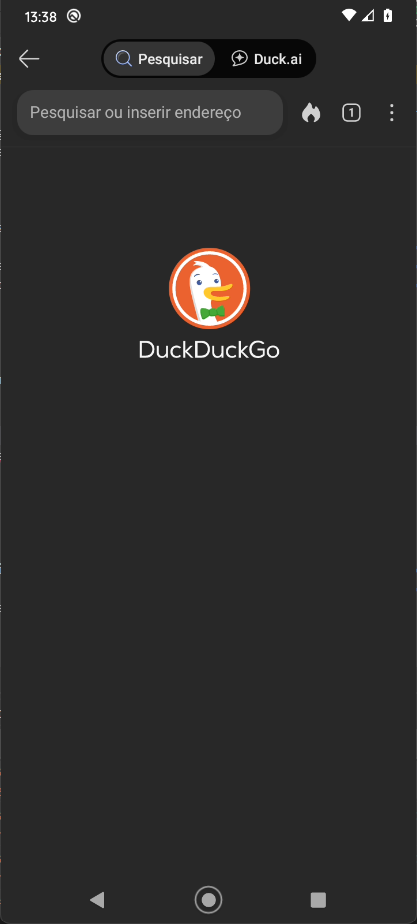
\includegraphics[trim={0cm 0cm 0cm 0cm}, clip, width=\textwidth]{imagens/duckduckgo_01.png}\\[0.2cm]
		\passo{DuckDuckGoOrange}{1}{Página inicial do DuckDuckGo}
	\end{minipage}
	\hfill
	\begin{minipage}{0.45\textwidth}
		\centering
		% Insira o print da opção Email Protection
		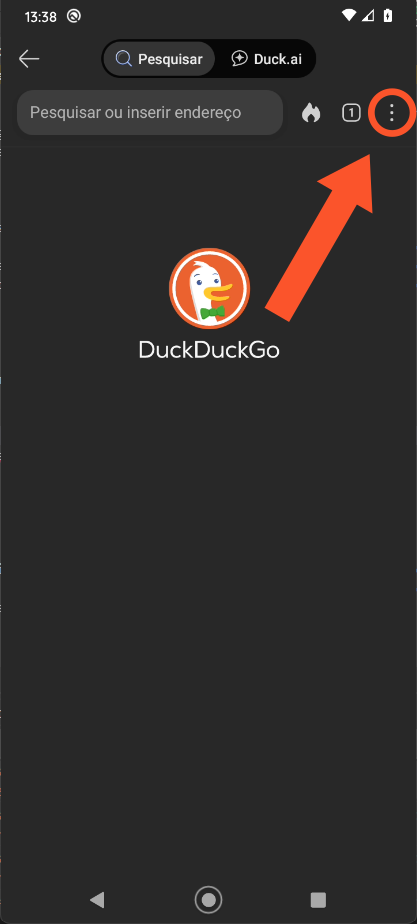
\includegraphics[trim={0cm 0cm 0cm 0cm}, clip, width=\textwidth]{imagens/duckduckgo_02.png}\\[0.2cm]
		\passo{DuckDuckGoOrange}{2}{Toque nos três pontinhos acima}
	\end{minipage}
\end{minipage}

\vspace{0.5cm}
\noindent
Feito a ação do \textbf{Passo 2} anterior, localize as \textbf{Definições} e toque nela como abaixo:

% --- BLOCO DE IMAGENS 2 ---
\noindent
\begin{minipage}{\textwidth}
	\centering
	\begin{minipage}{0.45\textwidth}
		\centering
		% Insira o print da tela de criar o endereço @duck.com
		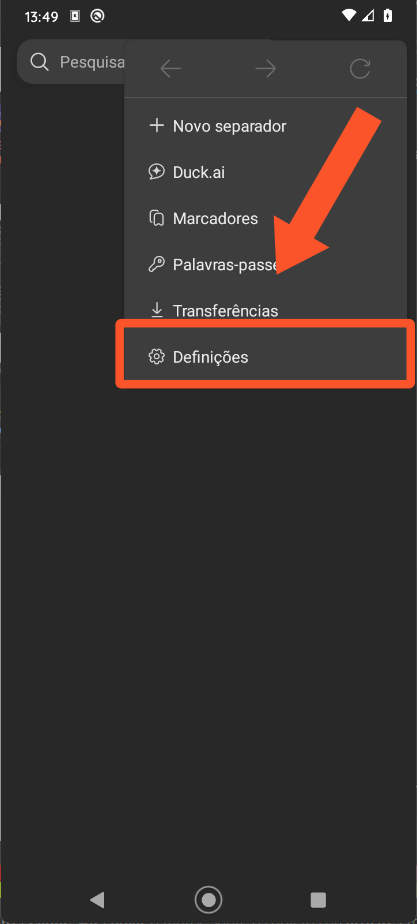
\includegraphics[trim={0cm 0cm 0cm 0cm}, clip, width=\textwidth]{imagens/duckduckgo_03.png}\\[0.2cm]
		\passo{DuckDuckGoOrange}{3}{Toque em \enquote{Definições}}
	\end{minipage}
	\hfill
	\begin{minipage}{0.45\textwidth}
		\centering
		% Insira o print de onde colocar o e-mail verdadeiro
		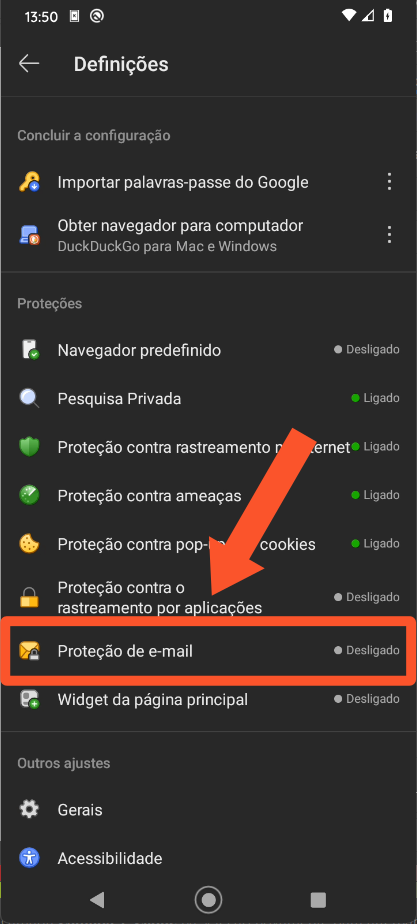
\includegraphics[trim={0cm 0cm 0cm 0cm}, clip, width=\textwidth]{imagens/duckduckgo_04.png}\\[0.2cm]
		\passo{DuckDuckGoOrange}{4}{Vá em \enquote{Proteção de e-mail}}
	\end{minipage}
\end{minipage}

\vspace{0.5cm}
\noindent
No \textbf{Passo 4} acima, note que a opção \enquote{Proteção de e-mail} está definida com \textbf{Desligado}. Então precisamos ligá-la, vamos fazer isso nos próximos passos.

% --- BLOCO DE IMAGENS 3 ---
\noindent
\begin{minipage}{\textwidth}
	\centering
	\begin{minipage}{0.45\textwidth}
		\centering
		% Insira o print da tela de criar o endereço @duck.com
		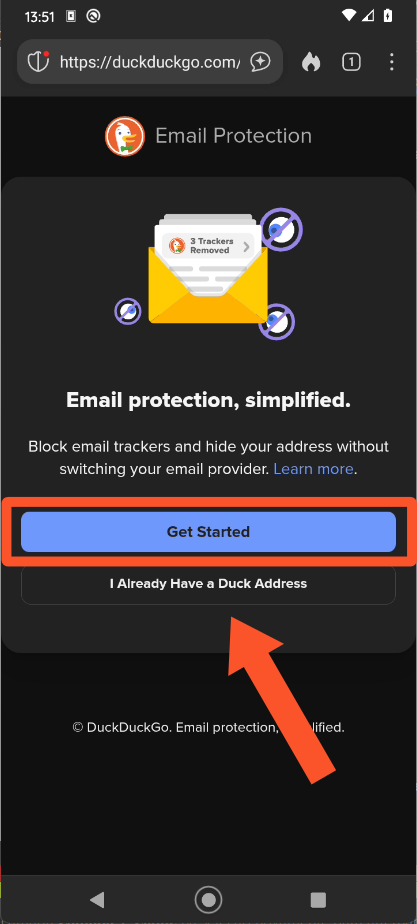
\includegraphics[trim={0cm 0cm 0cm 0cm}, clip, width=\textwidth]{imagens/duckduckgo_05.png}\\[0.2cm]
		\passo{DuckDuckGoOrange}{5}{Toque em \enquote{Get Started} (Comece)}
	\end{minipage}
	\hfill
	\begin{minipage}{0.45\textwidth}
		\centering
		% Insira o print de onde colocar o e-mail verdadeiro
		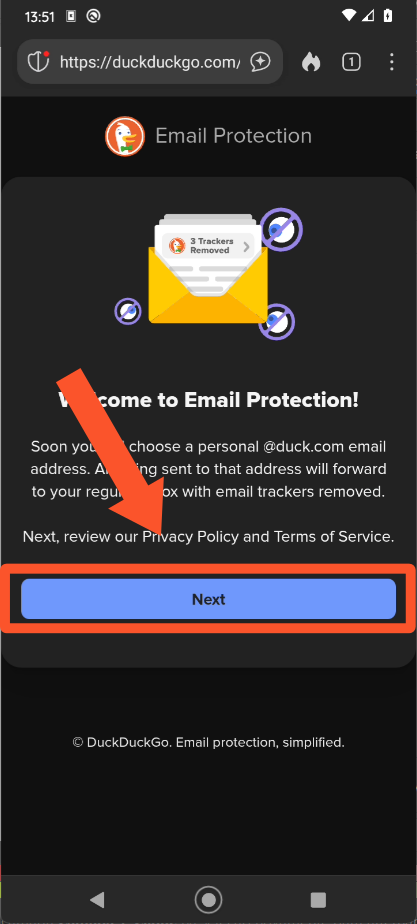
\includegraphics[trim={0cm 0cm 0cm 0cm}, clip, width=\textwidth]{imagens/duckduckgo_06.png}\\[0.2cm]
		\passo{DuckDuckGoOrange}{6}{Toque em \enquote{Next} (Próximo)} \newline
	\end{minipage}
\end{minipage}

\vspace{0.3cm}
\noindent

% --- BLOCO DE IMAGENS 4 ---
\noindent
\begin{minipage}{\textwidth}
	\centering
	\begin{minipage}{0.45\textwidth}
		\centering
		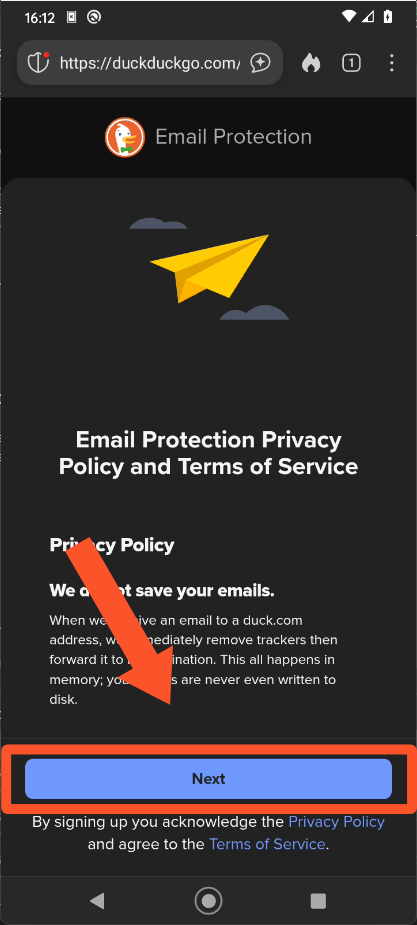
\includegraphics[trim={0cm 0cm 0cm 0cm}, clip, width=\textwidth]{imagens/duckduckgo_07.png}\\[0.2cm]
		\passo{BraveOrange}{7}{Toque no botão azul \enquote{Continue}}
	\end{minipage}
	\hfill
	\begin{minipage}{0.45\textwidth}
		\centering
		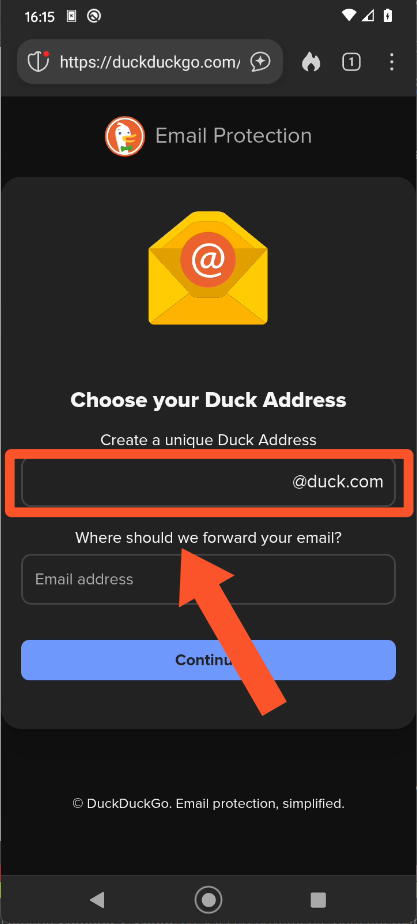
\includegraphics[trim={0cm 0cm 0cm 0cm}, clip, width=\textwidth]{imagens/duckduckgo_08.png}\\[0.2cm]
		\passo{BraveOrange}{8}{Escolha apenas o seu \enquote{Nome de Usuário}}
	\end{minipage}
\end{minipage}

\vspace{0.5cm}

\begin{tcolorbox}[colback=NordBackground, colframe=red, coltext=white, title=\faExclamationTriangle \ \textbf{Cuidado neste passo!}]
	\justifying \noindent
	No \textbf{Passo 8}, você deve digitar \textbf{APENAS} um nome (como se fosse um apelido):
	\begin{itemize}[label={}]
		\item \textbf{\textcolor{red}{\faTimesCircle \ ERRADO:}} \textbf{fulanodetal@gmail.com}
		\item \textbf{\textcolor{green}{\faCheckCircle \ CORRETO:}} \textbf{fulanodetal}
	\end{itemize}
	\noindent O final \textbf{@duck.com} já é colocado automaticamente pelo sistema. Não use espaços ou símbolos especiais.
\end{tcolorbox}

\vspace{0.3cm}
\noindent

% --- BLOCO DE IMAGENS 5 ---
\noindent
\begin{minipage}{\textwidth}
	\centering
	\begin{minipage}{0.45\textwidth}
		\centering
		% Insira o print da tela de criar o endereço @duck.com
		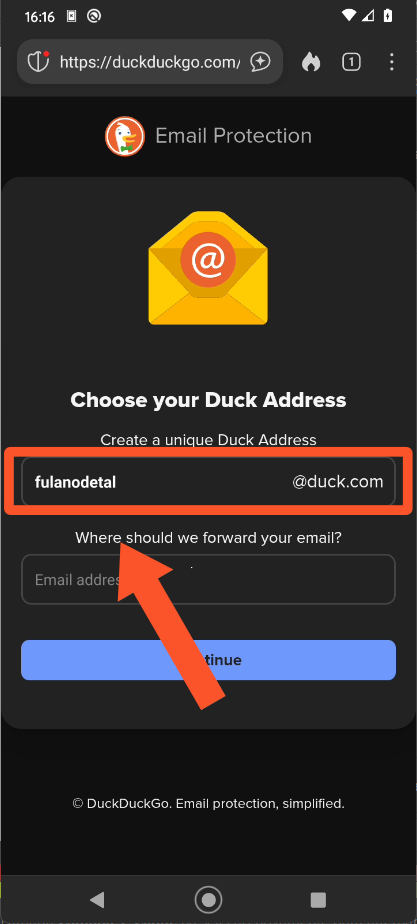
\includegraphics[trim={0cm 0cm 0cm 0cm}, clip, width=\textwidth]{imagens/duckduckgo_09.png}\\[0.2cm]
		\passo{DuckDuckGoOrange}{9}{Exemplo \textbf{CORRETO}} \newline
	\end{minipage}
	\hfill
	\begin{minipage}{0.45\textwidth}
		\centering
		% Insira o print de onde colocar o e-mail verdadeiro
		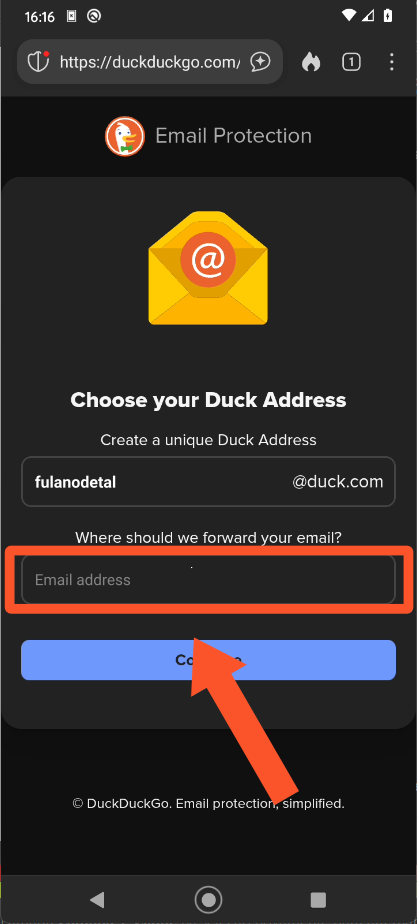
\includegraphics[trim={0cm 0cm 0cm 0cm}, clip, width=\textwidth]{imagens/duckduckgo_10.png}\\[0.2cm]
		\passo{DuckDuckGoOrange}{10}{Seu endereço de e-amil que pretende mascarar}
	\end{minipage}
\end{minipage}

\vspace{0.3cm}
\noindent

% --- BLOCO DE IMAGENS 6 ---
\noindent
\begin{minipage}{\textwidth}
	\centering
	\begin{minipage}{0.45\textwidth}
		\centering
		% Insira o print da tela de criar o endereço @duck.com
		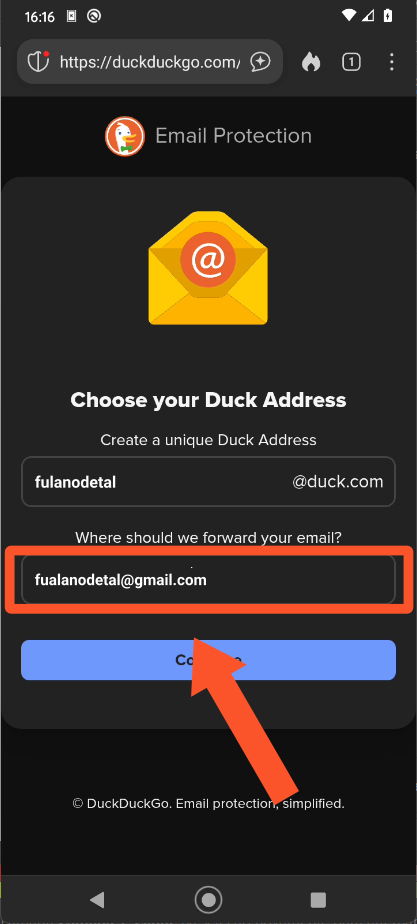
\includegraphics[trim={0cm 0cm 0cm 0cm}, clip, width=\textwidth]{imagens/duckduckgo_11.png}\\[0.2cm]
		\passo{DuckDuckGoOrange}{11}{Exemplo \textbf{CORRETO}}
	\end{minipage}
	\hfill
	\begin{minipage}{0.45\textwidth}
		\centering
		% Insira o print de onde colocar o e-mail verdadeiro
		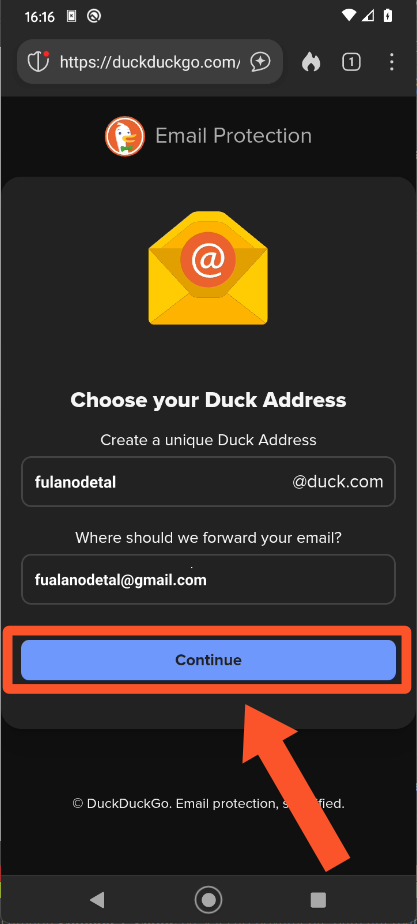
\includegraphics[trim={0cm 0cm 0cm 0cm}, clip, width=\textwidth]{imagens/duckduckgo_12.png}\\[0.2cm]
		\passo{DuckDuckGoOrange}{12}{Toque em \enquote{Continue}}
	\end{minipage}
\end{minipage}

\vspace{0.5cm}
\noindent
Muita atenção, no \textbf{Passo 13} abaixo o Duck vai perguntar se os valores que você digitou nos passo 11 e 9 estão corretos. Se sim, toque no botão azul \enquote{\textbf{This is correct}}. Acompanhe em seguida:

% --- BLOCO DE IMAGENS 7 ---
\noindent
\begin{minipage}{\textwidth}
	\centering
	\begin{minipage}{0.45\textwidth}
		\centering
		% Insira o print da tela de criar o endereço @duck.com
		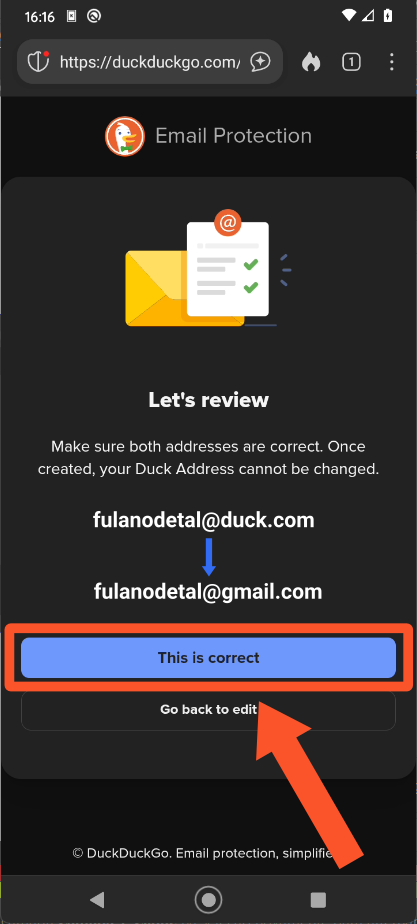
\includegraphics[trim={0cm 0cm 0cm 0cm}, clip, width=\textwidth]{imagens/duckduckgo_13.png}\\[0.2cm]
		\passo{DuckDuckGoOrange}{13}{Toque em \enquote{\textbf{This is correct}} (Está correto)}
	\end{minipage}
	\hfill
	\begin{minipage}{0.45\textwidth}
		\centering
		% Insira o print de onde colocar o e-mail verdadeiro
		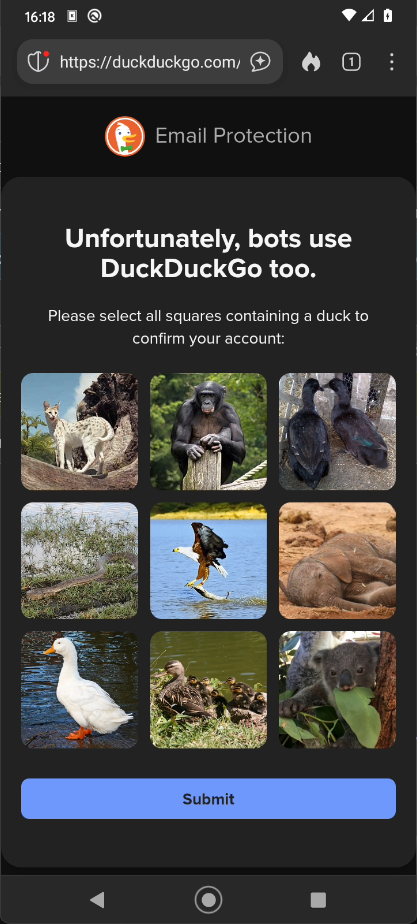
\includegraphics[trim={0cm 0cm 0cm 0cm}, clip, width=\textwidth]{imagens/duckduckgo_14.png}\\[0.2cm]
		\passo{DuckDuckGoOrange}{14}{Marque os patos nas imagens}
	\end{minipage}
\end{minipage}
% --- BLOCO DE IMAGENS 8 ---
\noindent
\begin{minipage}{\textwidth}
	\centering
	\begin{minipage}{0.45\textwidth}
		\centering
		% Insira o print da tela de criar o endereço @duck.com
		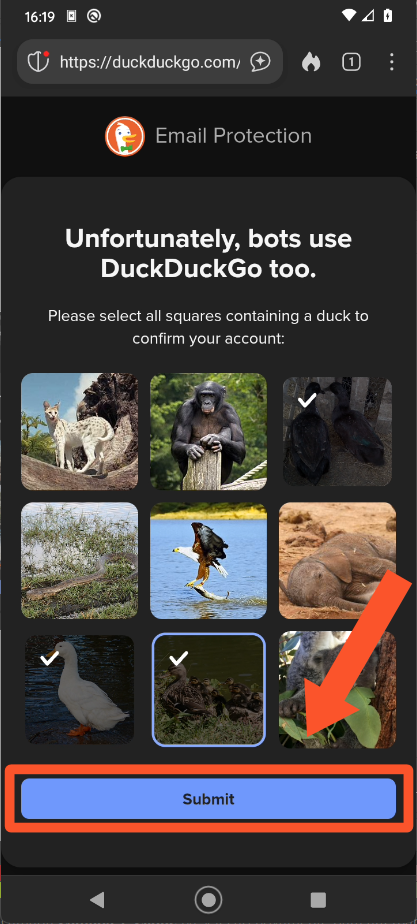
\includegraphics[trim={0cm 0cm 0cm 0cm}, clip, width=\textwidth]{imagens/duckduckgo_15.png}\\[0.2cm]
		\passo{DuckDuckGoOrange}{15}{Toque em \enquote{\textbf{Submit}} (Enviar)}
	\end{minipage}
	\hfill
	\begin{minipage}{0.45\textwidth}
		\centering
		% Insira o print de onde colocar o e-mail verdadeiro
		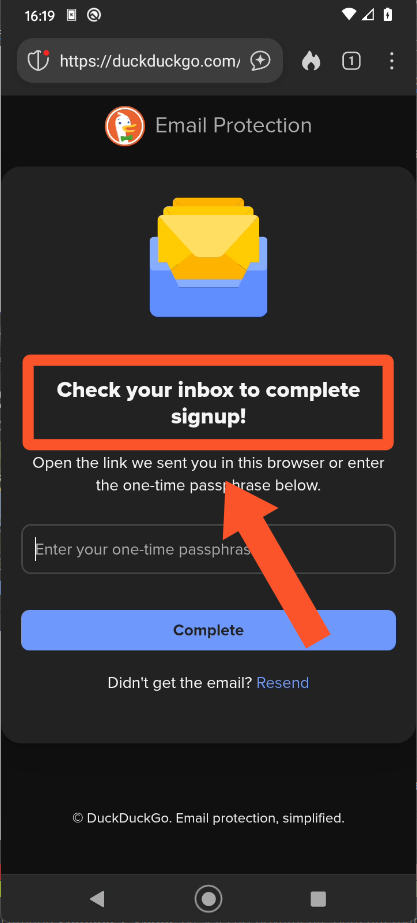
\includegraphics[trim={0cm 0cm 0cm 0cm}, clip, width=\textwidth]{imagens/duckduckgo_16.png}\\[0.2cm]
		\passo{DuckDuckGoOrange}{16}{O Duck enviou uma mensagem para seu e-email}
	\end{minipage}
\end{minipage}

\vspace{0.5cm}
\noindent
\textbf{Passo 16:} O DuckDuckGo enviará uma mensagem de confirmação para o seu e-mail real (aquele que você cadastrou no Passo 11, ex: \textbf{fulanodetal@gmail.com}). 

\vspace{0.3cm}

\begin{tcolorbox}[colback=NordBackground, colframe=red, coltext=white, title=\faExclamationTriangle \ \textbf{Cuidado com a Tradução Automática!}]
	\justifying\noindent
	O e-mail contém uma \textbf{frase de segurança} de 4 palavras (como: \textit{\textbf{thirsty krypton shush audition}}). 
	
	\vspace{0.3cm}
	\noindent
	\textbf{Atenção:} Essa frase \textbf{precisa ser digitada/colada em inglês}. Se o seu Gmail traduzir o e-mail automaticamente para o português, a frase não funcionará. 
	
	\vspace{0.3cm}
	\noindent
	\textbf{Como resolver:} Desative a tradução do navegador ou clique em \enquote{Mostrar original} no Gmail para copiar as palavras exatamente como elas foram enviadas.
\end{tcolorbox}

\vspace{0.3cm}
\noindent
Copie a frase em inglês, cole no campo indicado no aplicativo e clique no botão azul \textbf{\enquote{Complete}} para finalizar o seu escudo de e-mail. Veja no \textbf{Passo 17} abaixo como a mensagem deve ser:
\vspace{0.3cm}

% --- BLOCO DE IMAGENS 9 ---
\noindent
\begin{minipage}{\textwidth}
	\centering
	\begin{minipage}{0.45\textwidth}
		\centering
		% Insira o print da tela de criar o endereço @duck.com
		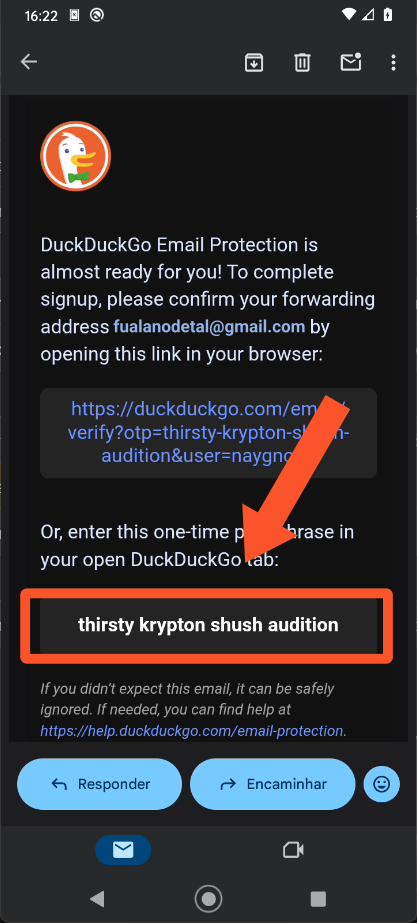
\includegraphics[trim={0cm 0cm 0cm 0cm}, clip, width=\textwidth]{imagens/duckduckgo_17.png}\\[0.2cm]
		\passo{DuckDuckGoOrange}{17}{No seu e-amil, copie a frase senha destacada}
	\end{minipage}
	\hfill
	\begin{minipage}{0.45\textwidth}
		\centering
		% Insira o print de onde colocar o e-mail verdadeiro
		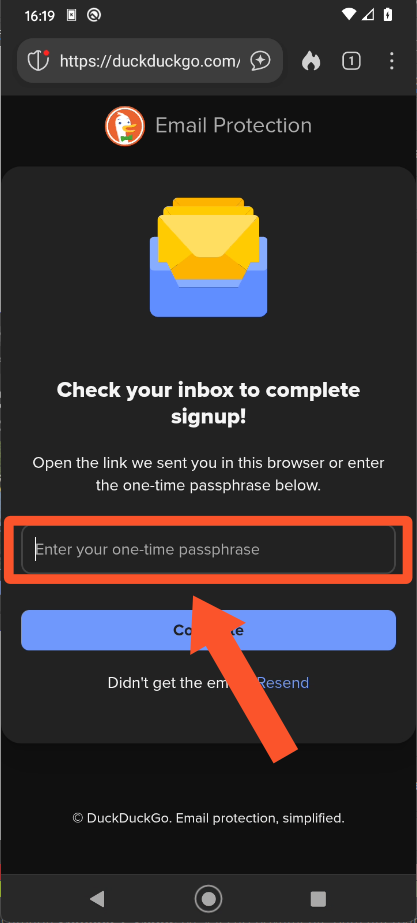
\includegraphics[trim={0cm 0cm 0cm 0cm}, clip, width=\textwidth]{imagens/duckduckgo_18.png}\\[0.2cm]
		\passo{DuckDuckGoOrange}{18}{No navegador DuckdDuckGo, digite/cole no campo destacado}
	\end{minipage}
\end{minipage}

\vspace{0.5cm}
\noindent
\textbf{Atenção:} A imagem do \textbf{Passo 17} acima mostra o conteúdo da mensagem enviada pelo serviço DuckDuckGo para o seu aplicativo de e-mail pessoal. Já a imagem do \textbf{Passo 18} ilustra o retorno à página do navegador para concluir a configuração. É fundamental não confundir o seu \textbf{aplicativo de e-mail} (onde você busca o código) com o \textbf{navegador} (onde você finaliza o cadastro).

% --- BLOCO DE IMAGENS 10 ---
\noindent
\begin{minipage}{\textwidth}
	\centering
	\begin{minipage}{0.45\textwidth}
		\centering
		% Insira o print da tela de criar o endereço @duck.com
		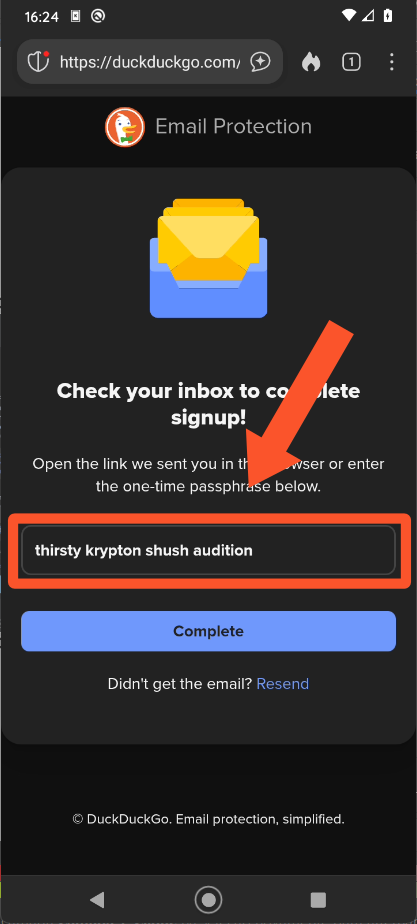
\includegraphics[trim={0cm 0cm 0cm 0cm}, clip, width=\textwidth]{imagens/duckduckgo_19.png}\\[0.2cm]
		\passo{DuckDuckGoOrange}{19}{Forma \textbf{CORRETA} (em inglês)}
	\end{minipage}
	\hfill
	\begin{minipage}{0.45\textwidth}
		\centering
		% Insira o print de onde colocar o e-mail verdadeiro
		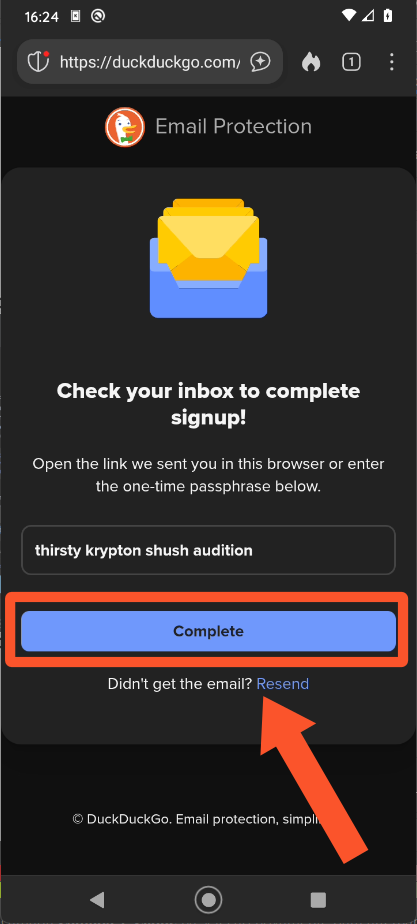
\includegraphics[trim={0cm 0cm 0cm 0cm}, clip, width=\textwidth]{imagens/duckduckgo_20.png}\\[0.2cm]
		\passo{DuckDuckGoOrange}{20}{Toque em \enquote{Complete}}
	\end{minipage}
\end{minipage}

\vspace{0.5cm}

% --- BLOCO DE IMAGENS 11 ---
\noindent
\begin{minipage}{\textwidth}
	\centering
	\begin{minipage}{0.45\textwidth}
		\centering
		% Insira o print da tela de criar o endereço @duck.com
		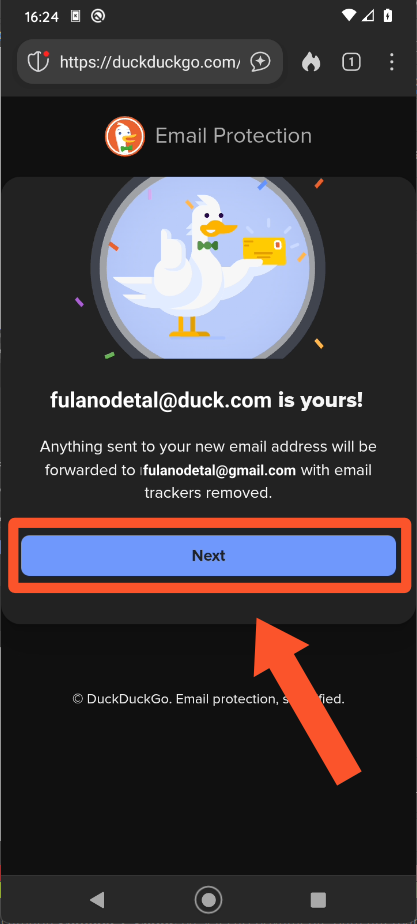
\includegraphics[trim={0cm 0cm 0cm 0cm}, clip, width=\textwidth]{imagens/duckduckgo_21.png}\\[0.2cm]
		\passo{DuckDuckGoOrange}{21}{Toque em \enquote{Next} (Próximo)}
	\end{minipage}
	\hfill
	\begin{minipage}{0.45\textwidth}
		\centering
		% Insira o print de onde colocar o e-mail verdadeiro
		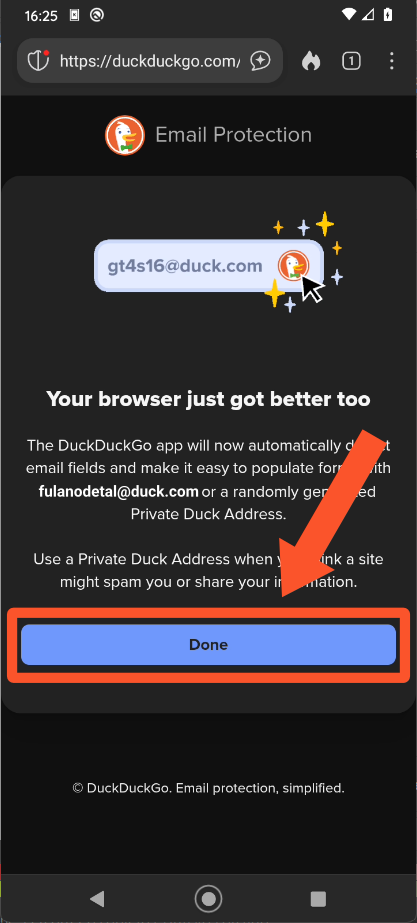
\includegraphics[trim={0cm 0cm 0cm 0cm}, clip, width=\textwidth]{imagens/duckduckgo_22.png}\\[0.2cm]
		\passo{DuckDuckGoOrange}{22}{Toque em \enquote{Done} (Feito)}
	\end{minipage}
\end{minipage}
\vspace{0.5cm}
% --- BLOCO DE IMAGENS 12 ---
\noindent
\begin{minipage}{\textwidth}
	\centering
	\begin{minipage}{0.45\textwidth}
		\centering
		% Insira o print da tela de criar o endereço @duck.com
		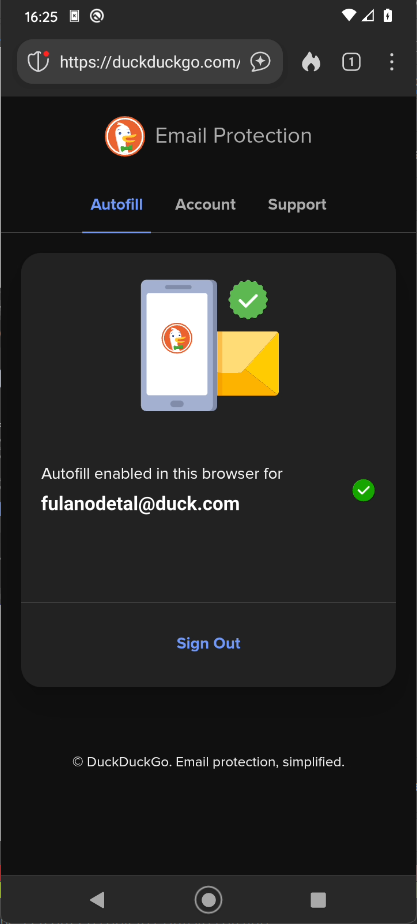
\includegraphics[trim={0cm 0cm 0cm 0cm}, clip, width=\textwidth]{imagens/duckduckgo_23.png}\\[0.2cm]
		\passo{DuckDuckGoOrange}{23}{Cadastro concluído com sucesso!}
	\end{minipage}
	\hfill
	\begin{minipage}{0.45\textwidth}
		\centering
		% Insira o print de onde colocar o e-mail verdadeiro
		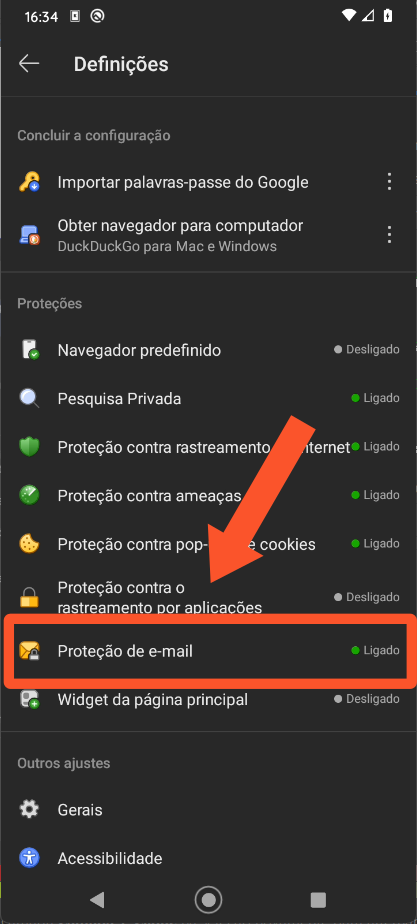
\includegraphics[trim={0cm 0cm 0cm 0cm}, clip, width=\textwidth]{imagens/duckduckgo_24.png}\\[0.2cm]
		\passo{DuckDuckGoOrange}{24}{Verifique se o status está \enquote{Ligado}}
	\end{minipage}
\end{minipage}

\vspace{0.5cm}
\noindent
Para confirmar que a proteção está ativa, acesse as \textbf{Definições} (conforme fizemos no Passo 4) e verifique se o campo \textbf{\enquote{Proteção de e-mail}} está marcado como \textbf{\textcolor{green}{Ligado}}, como demonstrado no \textbf{Passo 24}.


\section*{Usando uma Mascara de E-mail DuckDuckGo}

Acesse qualquer site que exija um e-mail de cadastro utilizando o navegador DuckDuckGo. Note na imagem do \textbf{Passo 25} que o ícone do \enquote{Patinho} aparecerá automaticamente dentro do campo de digitação:

\vspace{0.5cm}

% --- BLOCO DE IMAGENS 13 ---
\noindent
\begin{minipage}{\textwidth}
	\centering
	\begin{minipage}{0.45\textwidth}
		\centering
		% Insira o print da tela de criar o endereço @duck.com
		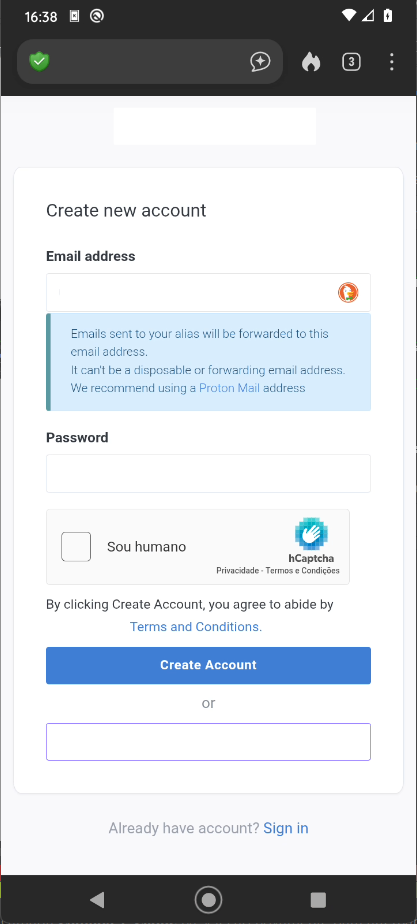
\includegraphics[trim={0cm 0cm 0cm 0cm}, clip, width=\textwidth]{imagens/duckduckgo_25.png}\\[0.2cm]
		\passo{DuckDuckGoOrange}{25}{Identifique o campo de e-mail}
	\end{minipage}
	\hfill
	\begin{minipage}{0.45\textwidth}
		\centering
		% Insira o print de onde colocar o e-mail verdadeiro
		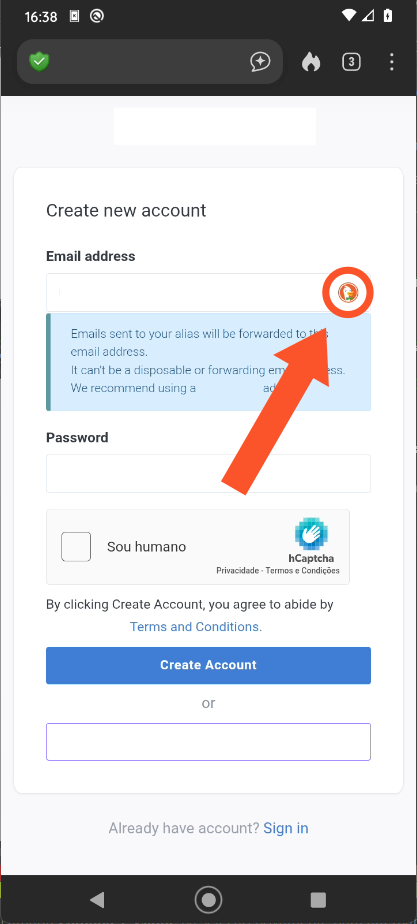
\includegraphics[trim={0cm 0cm 0cm 0cm}, clip, width=\textwidth]{imagens/duckduckgo_26.png}\\[0.2cm]
		\passo{DuckDuckGoOrange}{26}{Toque no ícone do \enquote{Patinho}}
	\end{minipage}
\end{minipage}

\vspace{0.3cm}
\noindent
Ao tocar no ícone, o navegador abrirá um \textbf{painel inferior} com as opções de proteção. Escolha a segunda opção para gerar um endereço totalmente novo, como indica o \textbf{Passo 27}:

% --- BLOCO DE IMAGENS 11 ---
\noindent
\begin{minipage}{\textwidth}
	\centering
	\begin{minipage}{0.45\textwidth}
		\centering
		% Insira o print da tela de criar o endereço @duck.com
		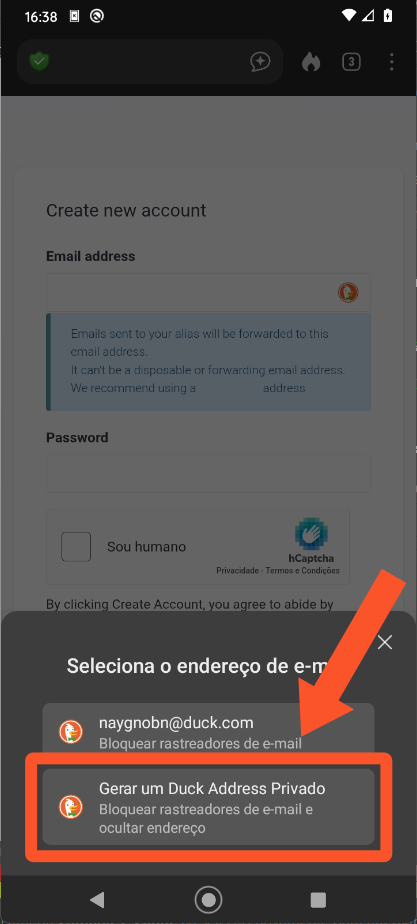
\includegraphics[trim={0cm 0cm 0cm 0cm}, clip, width=\textwidth]{imagens/duckduckgo_27.png}\\[0.2cm]
		\passo{DuckDuckGoOrange}{27}{Toque em \enquote{Gerer um Duck Address Privado}}
	\end{minipage}
	\hfill
	\begin{minipage}{0.45\textwidth}
		\centering
		% Insira o print de onde colocar o e-mail verdadeiro
		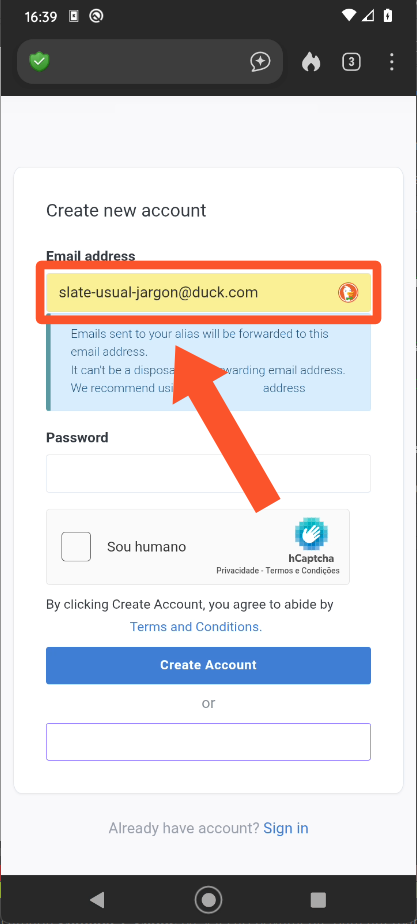
\includegraphics[trim={0cm 0cm 0cm 0cm}, clip, width=\textwidth]{imagens/duckduckgo_28.png}\\[0.2cm]
		\passo{DuckDuckGoOrange}{28}{O campo \textbf{Email address} é preenchido automaticamente}
	\end{minipage}
\end{minipage}

\vspace{0.5cm}
\begin{tcolorbox}[colback=NordBackground, colframe=DuckDuckGoOrange, coltext=white, title=\faMagic \ \textbf{Conforto e Segurança}]
	Pronto! Você se cadastrou no site sem revelar o seu e-mail verdadeiro. A partir de agora, o DuckDuckGo filtrará todos os rastreadores e entregará apenas o conteúdo limpo na sua caixa de entrada oficial.
\end{tcolorbox}

\vspace{0.5cm}
\noindent
\begin{tcolorbox}[colback=NordBackground, colframe=DuckDuckGoOrange, coltext=white, title=\faCheckCircle \ \textbf{Como usar no dia a dia?}]
	Após essa configuração, sempre que você estiver navegando e um site pedir o seu e-mail, o teclado do seu celular (ou o navegador) mostrará o ícone do Patinho. Basta tocar nele e o DuckDuckGo vai gerar um e-mail aleatório (exemplo: \textbf{potato-blue-iron@duck.com}) preenchendo o formulário para você automaticamente!
\end{tcolorbox}

\subsection*{\faEnvelope \ Outra Opção: \textcolor{SimpleLoginDarkPink}{SimpleLogin} (Proton)}
Se você busca uma ferramenta ainda mais robusta, conheça o \textbf{SimpleLogin} \cite{SimpleLogin2026}.

\vspace{0.3cm}
\begin{figure}[h]
	\centering
	
\includegraphics[width=0.4\textwidth]{imagens/simplelogin_dark_logo.png}
	\caption*{(\citeauthor{simplelogin_app} \citefield{simplelogin_app}{version} - Versão oficial)} % Texto manual imitando legenda
\end{figure}

\vspace{0.3cm}
\noindent \justifying %\RaggedRight % Usando RaggedRight para evitar buracos brancos
Ele faz parte do ecossistema da \textit{Proton} e permite criar e gerenciar máscaras de e-mail de forma profissional, inclusive permitindo que você responda e-mails usando a máscara, sem nunca revelar seu endereço real.

\vspace{0.3cm}
\noindent
\begin{center}
	\begin{minipage}{\linewidth}
		\begin{minipage}{0.3\linewidth}
			\centering
			\textbf{\textcolor{BraveOrange}{\faAndroid \ Android}}\\[0.2cm]
			\href{https://bfaxke.short.gy/simplelogin-android}{
				
\includegraphics[width=0.8\linewidth]{imagens/qr_simplelogin_android.png}
			}\\[0.1cm]
			{\scriptsize (Toque ou escaneie)}
		\end{minipage}
		\hfill
		\begin{minipage}{0.3\linewidth}
			\centering
			\textbf{\textcolor{NordText}{\faApple \ iOS / iPhone}}\\[0.2cm]
			\href{https://bfaxke.short.gy/simplelogin-ios}{
				
\includegraphics[width=0.8\linewidth]{imagens/qr_simplelogin_ios.png}
			}\\[0.1cm]
			{\scriptsize (Toque ou escaneie)}
		\end{minipage}
		\hfill
		\begin{minipage}{0.3\linewidth}
			\centering
			\textbf{\textcolor{BitwardenBlue}{\faGlobe \ Web}}\\[0.2cm]
			\href{https://bfaxke.short.gy/simplelogin-email}{
				
\includegraphics[width=0.8\linewidth]{imagens/qr_simplelogin_email.png}
			}\\[0.1cm]
			{\scriptsize (Online)}
		\end{minipage}
		
	\end{minipage}
\end{center}

%\begin{tcolorbox}[colback=NordBackground, colframe=BitwardenBlue, coltext=white, title=\faLightbulb \ \textbf{Outra Opção: SimpleLogin (Proton)}]
%	Se você busca uma ferramenta ainda mais robusta, conheça o \textbf{SimpleLogin} \cite{SimpleLogin2026}.
%	
%	\vspace{0.5cm}
%	\centering
%	
\includegraphics[width=0.4\textwidth]{imagens/simplelogin_dark_logo.png}
%	\caption*{(\citeauthor{simplelogin_app} \citefield{simplelogin_app}{version} - Versão oficial)}
	
%	\vspace{0.5cm}
%	\noindent \justifying
%	Ele faz parte do ecossistema da \textit{Proton} e permite criar e gerenciar máscaras de e-mail de forma profissional, inclusive permitindo que você responda e-mails usando a máscara, sem nunca revelar seu endereço real.
%\end{tcolorbox}
